\section{Introduction}
\subsection{Motivation}
Neurale netværk er rigtigt seje \cite{bishop2006}
\subsection{Proteins}
\subsubsection{What is}
\subsubsection{Secondary Structures}
\subsubsection{Solvent accessible surface area}
\subsection{Neural networks}
The common perception is that humans and animals process information, i.e. transform perceptional 
stimuli and physiological conditions into behaviour, by using their brains. This is imprecise 
however, as the brain as such is only one functioning part of what is called the \textit{nervous 
system}, which is in turn responsible for the internal workings of human and animal behaviour.

This nervous system is an abstaction over a number of \textit{neurons} interconnected by 
synapses. Neurons in turn are so-called electrically exitable cells. In a gross over-simplification, this can be translated into the case that each neuron can have different internal states, depending on the internal states of the neurons it is connected to, thus forming a \textit{neural network}.

\begin{figure}[h]
  \centering
  \frame{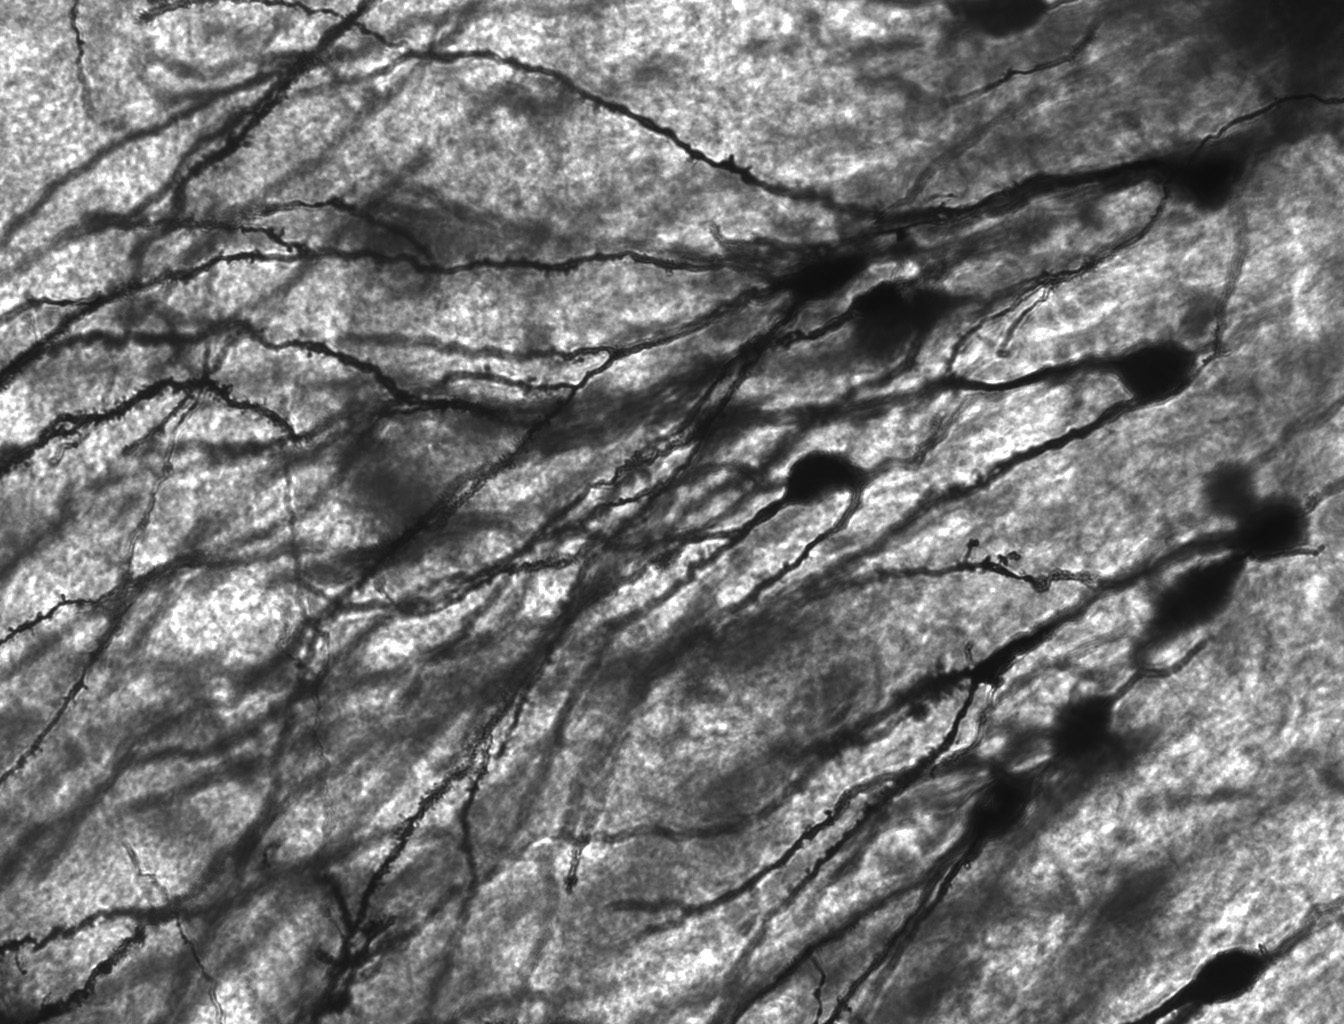
\includegraphics[width=0.8\linewidth]{images/Gyrus_Dentatus_40x}}
  \caption{Neurons in the dentate gyrus of an epilepsy patient.}
\end{figure}

While obviously interesting within the fields of biology or psychology, this structure has shown 
to be enourmously interesting in the field of computation, as one can in fact model this very 
thing and use it to make predictions based on prior observations, for example in regards to the 
aforementioned structures of proteins folding.

Analogously, or rather, digitally, we can use this model to construct an \textit{artificial 
neural network}.

These set themselves apart from biological neural networks in a couple of ways: most urgently in that while neurons in biological neural networks are connected to each other via synapses, so that each neuron has an either inhibitory or activating effect on whether or not a connected neuron 'fires', in artificial neural networks neurons are connected by \textit{edges}, each with an associated \textit{weight}, allowing the artificial networks to leave the discrete domain and enter the continuous.
\begin{tikzpicture}[line cap=round,line join=round,>=triangle 45,x=0.4cm,y=0.4cm]
\clip(-3.84,0.01) rectangle (18.8,18.55);
\draw [line width=1pt,fill=ffqqqq,fill opacity=1] (2,7) circle (0.4cm);
\draw [line width=1pt,fill=ffqqqq,fill opacity=1] (2,10) circle (0.4cm);
\draw [line width=1pt,fill=qqffqq,fill opacity=1] (7,4) circle (0.4cm);
\draw [line width=1pt,fill=qqffqq,fill opacity=1] (7,7) circle (0.4cm);
\draw [line width=1pt,fill=qqffqq,fill opacity=1] (7,10) circle (0.4cm);
\draw [line width=1pt,fill=qqffqq,fill opacity=1] (7,13) circle (0.4cm);
\draw [line width=1pt,fill=qqttcc,fill opacity=1] (12,10) circle (0.4cm);
\draw [line width=1pt,fill=qqttcc,fill opacity=1] (12,7) circle (0.4cm);
\draw [line width=1pt] (3,10)-- (6,13);
\draw [line width=1pt] (3,10)-- (6,10);
\draw [line width=1pt] (3,10)-- (6,7);
\draw [line width=1pt] (3,10)-- (6,4);
\draw [line width=1pt] (3,7)-- (6,13);
\draw [line width=1pt] (3,7)-- (6,10);
\draw [line width=1pt] (3,7)-- (6,7);
\draw [line width=1pt] (3,7)-- (6,4);
\draw [line width=1pt] (8,13)-- (11,10);
\draw [line width=1pt] (8,10)-- (11,10);
\draw [line width=1pt] (8,7)-- (11,10);
\draw [line width=1pt] (8,4)-- (11,10);
\draw [line width=1pt] (8,4)-- (11,7);
\draw [line width=1pt] (11,7)-- (8,7);
\draw [line width=1pt] (8,10)-- (11,7);
\draw [line width=1pt] (11,7)-- (8,13);
\end{tikzpicture}

\subsubsection{Convolutional neural networks}
\subsubsection{Multitask learning}